\documentclass[ngerman]{tudscrreprt}
\usepackage{selinput}
\SelectInputMappings{adieresis={ä},germandbls={ß}}
\usepackage[T1]{fontenc}
\usepackage{babel} \usepackage{isodate}
\usepackage{amssymb}
\usepackage{amsmath}
\usepackage{nccmath}

\usepackage{float} % lädt das Paket zur Verwendung von zusätzlichen Positionsbefehlen
\usepackage{wrapfig}  
\usepackage{picinpar}   
\usepackage{enumerate}
\usepackage{hyperref}

\begin{document}
\faculty{Fakultät Elektrotechnik und Informationstechnik} \department{} \institute{INSTITUT FÜR REGELUNGS- UND STEUERUNGSTHEORIE} \chair{} \title{NICHTLINEARE REGELUNGSTECHNIK 1\\ Dr.-Ing. J. Winkler
}
% \thesis{diss}
% \degree[Dr.-Ing.]{Doktor-Ingenieur}
\author{Mitschrift von Bolor Khuu}
% \dateofbirth{2.1.1990}
% \placeofbirth{Dresden}
\date{\today}
% \defensedate{20.10.2014}
% \referee{Dagobert Duck \and Mac Moneysac}
\maketitle
\tableofcontents
\newpage
\chapter{Grundbegriffe und Eigenschaften nichtlinearer Systeme}
\section{Nichtlineare Übertragungsglieder}
Anordnung, die aus einem Eingangssignal $u(t)$ ein Ausgangssignal $y(t)$ erzeugt. \\$y(t)$ mit Operator~$\varphi.$ \hspace{1cm} $y(t)=\varphi(t)$ \newline
\begin{itemize}
\item \textbf{Beispiel:} \\ $y(t)=\int\limits_{0}^t u(\tau) d\tau$  \hspace{1cm}
\medskip
$\varphi \rightarrow$  Ausführungs der Integration

$\varphi(u+u^*)=\varphi(u)+\varphi(u^*).$ \\
$\varphi(c\cdot u) = c \cdot \varphi(u). $ \\
$\varphi(c\cdot u+ c^* \cdot u^*) = c\cdot \varphi(u) + c^* \cdot \varphi(u^*).$
\bigskip
\\
\item \textbf{Beispiel 1:}
\begin{eqnarray*}
y &=& \varphi(\underline{u}) \hspace{1cm} \underline{u} \in \mathbb{R}^2 \nonumber \\
  &=& u_{1}\cdot u_{2} \hspace{0.7cm} y \in \mathbb{R}
\end{eqnarray*}
$\varphi(\underline{u} + \underline{u}^*) = \varphi {u_{1} + u_{1}^* \choose u_{2} + u_{2}^* }$
$\hspace{1cm} \underline{u} = {u_{1} \choose u_{2}}$
$\hspace{1.7cm} = (u_{1} + u_{1}^*) \cdot (u_{2} + u_{2}^*)  $
$\hspace{1.7cm} = \underbrace{u_{1}\cdot u_{2}}_{\varphi(u)} + \underbrace{u_{1}^* \cdot u_{2}^*}_{\varphi(u^{*} )} + u_{1}\cdot u_{2}^* + u_{1}^* u_{2}$
$\rightarrow$ nicht linear
\\ 
\item \textbf{Beispiel 2:}
\newline
$y = m\cdot u + b =: f(u). \quad u,y,m,b \in \mathbb{R}$ \bigskip \newline
$
\begin{matrix}
\varphi(u+u^*) & = & m (u + u^*) + b. \\
               & = & m u + b + m u^*\\
               & = & \varphi(u) + \underbrace{m u^*}_{\text{nicht linear}\rightarrow \text{affin in } u } 
\end{matrix}
$
\item \textbf{Errinerung:} Ein Übertragungsglied heißt zeitinvariant wenn für dieses das Verschiebungsprinzip gilt.\\
$
\begin{matrix}
y(t) = \varphi( u (t) ) & u & \mbox{ -in $t_{0}$ nach rechts schieben}\\
& u(t-t_{0})&
\end{matrix}
$
\\
$\rightarrow \varphi(\,u(t-t_{0})) = y(t-t_{0}) \rightarrow y$ auch um $t_{0}$ nach verschob.
\\
\item \textbf{Folgerung:}
Da das Überlagerungsprinzip bei nicht linearen Systemen nicht gilt , läßt nicht der Zusammenhang zwischen den Ein und Ausgangsgrößen nicht durch ein Faltungsintegral darstellen.
\item \textbf{Folge:}
\begin{itemize}
\item keine komplexen Übertragungsfunktionen 
\item kein Freqünzgang 
\item kein Laplace-Transformation.
\end{itemize}
$\rightarrow$ Hilfsmittel der komplexen Funktionentheorie nicht anwendbar!!\\
$\rightarrow$ keine allgemein gültige Theorie$\rightarrow$ Behandlung bestimmbar Systemklassen.\\
$\rightarrow$ Systemtheoretische Eigenschaften, die für einen Unterraum des $\mathbb{R}^n$ entwickelt wurden, gelten nicht notwendigerweise für den vollständigen $\mathbb{R}^n$ lokale und globale Eigenschaften fallen nicht zusammen.
\end{itemize}
\section{Typische Phänomene in nichtlinearen Systeme}
\subsubsection{Linearer Fall (Errinerung)}
lineares System 
\begin{equation*}\dot{x} = A\cdot x , \quad x(0) = x_{0} \quad x, x_{0} \in \mathbb{R}^{n}\quad A  \in \mathbb{R}^{n\times n}
\tag{1.3}
\label{eq:1.3}
\end{equation*} 
\\
\textbf{Ruhelagen}: Lösung von $A\cdot x = 0.$\\
\begin{itemize}
\item wenn $A$ regulär $(\det A\ne 0)$ dann gibt es genau eine Ruhelage $x_{e}$ mit $A\cdot x_{e}=0$ und $x(t_{0})=x_{e} \rightarrow x(t)=x_{e} \quad \forall \, t > t_{0}$
\item wenn $A$ singulär $(\det{A} = 0)$ dann gibt es unendlich viele Ruhelagen.
\item Die Lösung des Anfangswertproblems (\ref{eq:1.3}) lautet mit der\\ Transitionsmatrix $\varphi(t)=e^{A\cdot t} = \underline{T} + A\cdot t + \frac{1}{2} \cdot A^2 \cdot t^2 $ wie folgt 
$x(t) = \phi(t)\cdot x_{0}$ \\ Damit gilt:\\ $a_{1}\cdot e^{-\alpha \cdot t} \leq \parallel x(t) \parallel \leq a_{2}\cdot e^{\alpha_{2} \cdot t} \qquad \text{ mit }a_{1}, a_{2}, \alpha_{1}, \alpha_{2} > 0.$
\item Die Ruhelage $x_{e}$ ist asymptotisch stabil. Wenn alle Eigenwerte von $A$ einen negativen Realteil haben und unabhängig von den Angangsbedinungen.
\item wenn 
\begin{equation}
\dot{x} = A\cdot x + B\cdot u \quad x(0) = x_{0}
\qquad B \in \mathbb{R}^{n\times m}, u \in \mathbb{R}^{m}
\tag{1.4}
\label{eq:1.4}
\end{equation}
Asymptotisch Stabilität von $\dot{x}= A\cdot x $ impliziert BIBO -Stabilität von (\ref{eq:1.4})
\item sinusformiges Eingangssignal $\rightarrow$ sinusförmiges Ausgangssignal
\end{itemize}
\subsubsection{Nichtlinearer Fall}
\begin{enumerate}[(A)]
\item \textbf{Mehrfache Ruhelage (Gleichgewichtspunkte)}. \\
Nichtlinearer System , keine , eine, mehrere , unendliche viele Ruhelagen die auch abhängig von den Anfangsbedingung sein können.
\\ \textbf{Ruhelagen:} $x_{e}: \quad x(0) = x_{e} \rightarrow x(t) = x_{e} ~\forall \,~ t>0.$  
\begin{itemize}
\item\textbf{Beispiel:} $\dot{x} = -x + x^2 \quad x(0)= x_{0} \quad x \in \mathbb{R}$
\\
Lösung: $x(t)= \frac{x_{0} \cdot e^{-t}}{1- x_{0} + x_{0}\cdot e^{-t} }$
\begin{figure}[H] 
  \centering 
  \def\svgwidth{200pt} 
  %\input{Zeichnung.pdf_tex} 
  \input{bild112.pdf_tex} 
\end{figure} 
\end{itemize}
\item \textbf{Endliche Fluchtzeit}
\\
Die Trajektorie eines nichtlinearen Systems kann in endlicher Zeit gegen $\infty$ oder in die Ruhelage laufen.
\begin{itemize}
\item\textbf{Beispiel:} siehe \textbf{A.} mit $x_{0}>1$\\
$\dot{x} = - \sqrt{x} \quad x_{0} > 0. \quad $ \\
\[ x(t) = \left\{ 
  \begin{array}{l l}
    (\sqrt{x_{0}} - \frac{t}{2})^2 & \quad \text{für $0\leq t \leq 2\cdot \sqrt{x_{0}}$}\\
    0 & \quad \text{sonst}
  \end{array} \right.\] 
\\
\textbf{Ruhelage:} $x_{e}= 0 $ in endlicher Zeit wird die Ruhelage aus jedem beliebig möglichichen Anfangszustand erreicht.
\end{itemize}
\item\textbf{Grenzzyklen}\\
Anfangswert unabhängige Dauerschwingungen konstante Amplitude und $T-$Periodendauer ohne äußere Anregung.
\begin{itemize}
\item \textbf{Beispiel:}\\
van der Pol-Gleichung\\
$m\ddot{x} + 2c\cdot (x^2 -1)\cdot \dot{x} + k x = 0, \quad m,c,k > 0. \\$
(Feder Masse System mit posivit abhängige Dämpung $2c\cdot (x^2 - 1)$ ~~)\\
$\rightarrow x\gg 1 $ Positive Dämpung, Energieverlust konvergierendes Verhalten.\\
$\rightarrow x\ll 1 $ Negative Dämpung, divirgierendes Verhalten.  \\
weder unbegrenztes Wachstum , nach Konvergenz gegen 0.
\begin{figure}[H]  
  \centering
  \def\svgwidth{200pt} 
  %\input{Zeichnung.pdf_tex} 
  \input{sincos.pdf_tex} 
\end{figure} 
\end{itemize}
\end{enumerate}
\section{Lipschitz-Bedingung und Stetigkeit}
\begin{itemize}
\item \textbf{Satz:}
Sind die Funktionen $f(x,t)$ aus (1.7) und $\frac{\partial F}{\partial x} (x, t)$ auf der Menge $B\times \left[t_0, t_0 + \delta \right] \text{ mit } B \in \mathbb{R}^n$ stetig dann erfüllt $f(x,t)$ lokal Lipschitz-Bedingung (1.8) 
\begin{itemize}
\item $f(x,t)$ nicht stetig differenzierbar $\rightarrow f(x,t)$ kann durchaus Lipschitz-Stetig sein.
\end{itemize}
\item \textbf{Satz:} Globale Exitenz und Eindeutigkeit
\begin{itemize}
\item Ausgangspunkt: \\$f(x,t)$ aus (1.7) ist stückweise stetig int t, global Lipschitz $\forall \, t \in [t_0 , t_0 + \tau] \Rightarrow$ (1.7) hat eine Lösung im Zeitintervall $[t_0 , t_0 + \delta]$\\
Sind $f(x,t)$ und $\frac{\partial F}{\partial x} (x,t) $ auf $\mathbb{R}^n \times [t_0, t_0 + \tau] $ stetig, dann ist $f(x,t) $ global Lipschitz, wenn $\frac{\partial f}{\partial x} (x,t) \text{ auf } \mathbb{R}^n \times [ t_0 , t_0+\tau] $ gleichmässig beschränkt ist.
\item Gleichmässig beschränkt:\\ $\frac{\partial f}{\partial x} (x,t) $ ist gleichmässig beschränkt, wenn gilt. Zu jeder positiv finiten Konstante $a$ existiert ein $\beta(a) $ mit unabhängig von $t_0$!\\
$
\left|\left| \frac{\partial f}{\partial x}(x(t_0) , t_0) \right| \right| \leq a \Rightarrow
\left|\left| \frac{\partial f}{\partial x} (x(t) , t) \right|\right| \leq \beta(a) \quad \forall \, t\in[t_0, t_0+\tau], x\in \mathbb{R}^n\\
$
\end{itemize}
\begin{itemize}
\item \textbf{Beispiel:}\\ 
$\left.
\begin{matrix}
\dot x_1 &=& - x_1 + x_1 \,x_2 \\
\dot x_2 &=& \,x_2 + x_1 \, x_2 
\end{matrix}\right\} f(x) \rightarrow  \frac{\partial f}{\partial x} = 
\begin{pmatrix}
-1 + x_2 & x_1 \\
-2 + x_2 & 1 - x_1
\end{pmatrix} \quad f(x)
$ 
ist nicht stetig differenzierbar, $\Rightarrow$ \textbf{\textit{lokal Lipschitz}}\\
gleichmässig beschränkt? \\
$
\left|\left| 
\begin{pmatrix}
-1 + x_2 & x_1 \\
-2 + x_2 & 1 - x_1
\end{pmatrix}
\right|\right|_\infty = \max{ \left\{  \left|-1 + x_2\right|, \, \left|x_2\right| + \left|1-x_1\right| \right\} }\\
\Rightarrow
$ nicht gleichmässig beschränkt, nicht global Lipschitz.
\item \textbf{Beispiel:}
\\
$\left. 
\begin{matrix}\dot{x_{1}} &=& -x_{1} + x_{1}\cdot x_{2}\\
\dot{x_{2}} &=& x_{2} - x_{1}\cdot x_{2}\end{matrix} \right\} f(x) $
\\
$\frac{\partial{f}}{\partial{x}} = \bordermatrix{& & \cr & -1+x_{2} & x_{1} \cr 
                                                 & -x_{2} & 1-x_{1} \cr}$
$\qquad \left.
\begin{matrix}
f(x) &\rightarrow& \text{ stetig differenzierbar}\\
\frac{\partial{f}}{\partial{x}} & \rightarrow& \text{ nicht global Lipschitz }
\end{matrix}
\right\} f \text{ ist lokal Lipschitz}
$\\
$\left|\left| \bordermatrix{& & \cr & -1+x_{2} & x_{1} \cr 
                                                 & -x_{2} & 1-x_{1} \cr} \right|\right| _{\infty} = \Bigg\{|-1+x_{2}| + |x_{1}|, |x_{2}| + |1-x_{1}| \Bigg\} $

\end{itemize}
\end{itemize}
\chapter{Analyse nichtlinearer Systeme 2. Ordnung in der Phasenebene bzw, Nähe ihrer Ruhelagen, Phasenportraits}
\section{Einführung-Motivation}
System der Form\\
\begin{equation}
\dot x_1 =f_1(x_1,x_2) \quad x_1(0)=x_{10} \quad \tag{2.1a}
\end{equation}
\begin{equation}
\dot x_2 = f_2(x_1,x_2) \quad x_2(0)=x_{20} \quad \tag{2.1b}
\end{equation}
\label{sec:2.1}
$
\text{ mit } x_1, x_2 \in \mathbb{R}$ Phasenebene $x_1 - x_2-$Ebene
\\Lösung von (\ref{sec:2.1}) liefert $x(t) = (x_1(t), x_2(t))^T$ anschaulich darstellbar in der Ebene!
Rechte Seite von (\ref{sec:2.1}) Tangentenvektor an der jeweiligen Lösungskurve. Jedem Punkt ist eindeutig ein Vektor $f(x) = (f_1(x), f_2(x))^T$zugeordnet.\\
\textit{Ziel}: Konstruktion von Phasenportraits
\begin{itemize}
\item Menge von Anfangswerten in der $x_1 - x_2$-Ebene
\item Trajektorien berechnen $\hat{=}$ Lösung von \ref{sec:2.1}
\item Familie von Trajektorien $=$ Phasenprotrait, Zeitinformation geht verloren
\begin{figure}[H]  
  \centering
  \def\svgwidth{220pt} 
  %\input{Zeichnung.pdf_tex} 
  \input{phasenport000.pdf_tex} 
\end{figure} 
\end{itemize}
\section{Qualitatives Verhalten linearer System}
linearisiertes System (2.1) um die Ruhelage $x_{1e}, x_{2e}\\
\dot{\tilde x} = A\, \tilde x \text{ mit } 
A= \underbrace{\left.\begin{pmatrix}
\frac{\partial f_1}{\partial x_1} & \frac{\partial f_1}{\partial x_2} \\
\frac{\partial f_2}{\partial x_1} & \frac{\partial f_2}{\partial x_2} 
\end{pmatrix}\right|_{x_{1e}, x_{2e}}}_{\text{\textbf{Jakobi-Matrix}}} \qquad \tilde x = \binom{x_1 - x_{1e}}{x_2 - x_{2e}}\\
A$ läßt sich in Jordan Normalform transfonieren.(RT2)\\
$z= T\cdot x \qquad \rightarrow \dot z = T^{-1} \cdot A \cdot T \cdot z = J\cdot z \\A$ habe die Eigenwerte $\lambda_1, \lambda_2$. Dann gibt's 4 Fälle
\begin{itemize}
\item \textbf{A).} 
$J=
\begin{pmatrix}
\lambda_1 & 0\\
0 & \lambda_2
\end{pmatrix} \qquad \text{2 Verschiedene reelle Eigenwerte}
$
\item\textbf{B).} 
$J=
\begin{pmatrix}
\lambda & 0\\
0 & \lambda
\end{pmatrix} \qquad \text{~~1 Doppelter Eigenwerte } \lambda \in \mathbb{R} 
$
\item\textbf{C).} 
$J=
\begin{pmatrix}
a & -b\\
b & a
\end{pmatrix} \qquad \text{1 konjugiert komplexe Eigenwertpaar } \lambda = a \pm jb 
$
\item\textbf{D).} Spezialfall: 
mindestens $1$ Eigenwert ist $0$ Fall A). Beide Eigenwerte reell, $A$ ist diagonalähnlich 
$ 
\dot z=
\begin{pmatrix}
\lambda_1 & 0\\
0 & \lambda_2
\end{pmatrix} \qquad 
z(0)=
\begin{pmatrix}
z_{10}\\
z_{20}
\end{pmatrix}\\
$ 
\begin{equation}
\boxed{\left\{
\begin{matrix}
\dot z_1(t) &=& \lambda_1 z_1(t)\\
\dot z_2(t) &=& \lambda_2 z_2(t)
\end{matrix}
\right. }
\quad
\Rightarrow 
\boxed{\left\{
\begin{matrix}
\dot z_1(t) &=& z_{10} \,e^{\lambda_1 t}\\
\dot z_2(t) &=& z_{20} \,e^{\lambda_2 t}
\end{matrix}
\right.
}
\tag{2.2}
\end{equation}
$ 
\text{Eliminieren von } t:
\frac{1}{\lambda_1} \ln{ \frac{z_1}{z_{10}}} = \frac{1}{\lambda_2} \ln{ \frac{z_2}{z_{20}}}\qquad
$ 
\begin{equation}
\boxed{z_2 = \frac{z_{20}}{z_{10}^{(\frac{\lambda_2}{\lambda_1} )}} z_1^{(\frac{\lambda_2}{\lambda_1})}
}
\tag{2.3}
\end{equation}
\begin{align}
\boxed{\text{ Steigung:}\qquad
\frac{d z_2}{d z_1} = \frac{z_{20}}{z_{10}^{\lambda_2/\lambda_1}} \frac{\lambda_2}
{\lambda_1} z_1^{ \frac{\lambda_2}{\lambda_1} - 1 }
}
\tag{2.4}
\end{align}
\item $\lambda_2 < \lambda_1 < 0 \qquad (\lambda_2 = \text{ schnell } , \lambda_1 = \text{ langsam })\\
|z_1| \rightarrow 0 \qquad ~\Big|\frac{d z_1}{d z_2}\Big|\rightarrow 0\\
|z_1| \rightarrow \infty \qquad \Big|\frac{d z_1}{d z_2}\Big|\rightarrow \infty \\
$
\begin{figure}[H]  
  \centering
  \def\svgwidth{300pt} 
  %\input{Zeichnung.pdf_tex} 
  \input{phasenport00.pdf_tex} 
\end{figure} 
$v_i$ die durch den zum Eigenwert $\lambda_i$ gehörigen Eigenvektor definierte Richtung
\item $\lambda_2 > \lambda_1 > 0$ instabile Knoten \\wie stabile Knoten,nur Pfeile andersum
\item $\lambda_2 < 0 < \lambda_1 \quad \left.
\begin{matrix}
z_1(t) &=& z_{10}\cdot e^{\lambda_1 t} \rightarrow \infty \\
z_2(t) &=& z_{20}\cdot e^{\lambda_2 t} \rightarrow 0 
\end{matrix}
\right\}$ für $t\rightarrow \infty$ 
\begin{figure}[H]  
  \centering
  \def\svgwidth{300pt} 
  %\input{Zeichnung.pdf_tex} 
  \input{phasenport01.pdf_tex} 
\end{figure}
\item konjugiert komplexer Fall $\lambda = a \pm jb$
\begin{figure}[H]  
  \centering
  \def\svgwidth{300pt} 
  %\input{Zeichnung.pdf_tex} 
  \input{phasenport02.pdf_tex} 
\end{figure} 
\end{itemize} 
\section{Qualatatives Verhalten nichtlinearer Systeme in der Nähe ihrer Ruhelage}
\begin{equation}
\dot x_1 = f_1(x_1,x_2)\quad x_1(0) = x_{10} \quad \dot x_2 = f_2(x_1,x_2)\quad x_2(0)=x_{20} \quad
\tag{2.6}
\label{eq:2.6}
\end{equation}
$\text{Taylor-Reihen-Entwicklung um Ruhelage }(x_{1e}, x_{2e})\\
\dot x_i = \underbrace{f_i (x_{1e}, x_{2e}) }_{=0}+ \left. \frac{\partial f_i}{\partial x_1}\right|_{(x_{1e}, x_{2e})}(x_1 - x_{1e}) + \left. \frac{\partial f_i}{\partial x_2}\right|_{(x_{1e}, x_{2e})}(x_2 - x_{2e}) + \text{ T.h.O}\\
$
\begin{equation}
\begin{pmatrix}
\dot{\tilde{x}}_1\\
\dot{\tilde{x}}_2
\end{pmatrix}=\left.
\begin{pmatrix}
\frac{\partial f_1}{\partial x_1}& \frac{\partial f_1}{\partial x_2} \\
\frac{\partial f_2}{\partial x_1}& \frac{\partial f_2}{\partial x_1}
\end{pmatrix}\right|_{(x_{1e}, x_{2e})} \cdot
\begin{pmatrix}
\tilde{x}_1\\
\tilde{x}_2
\end{pmatrix} \qquad \tilde x_i = x_i - x_{ie}
\tag{2.7}
\end{equation}
\begin{itemize}
\item \textbf{\textit{Satz von Hartmann-Grobmann}}\\
Wenn die \ref{eq:2.6} gehörige Jakobi-Matrix keine Eigenwerte mit verschwindenden Realteil hat, so existiert ein Homöomorphismus in der Umgebung $U$ um die Ruhelage zwischen den Trajektorien des nichtlinearen Systems $\dot x = A\cdot \tilde x \qquad h: U\rightarrow \mathbb{R}^2$\\Ruhelagen, deren Jacobi-Matrix Eigenwerte mit nicht verschwindend Realteil haben heißen hyperbolisch. Jordan-Form im Falle eines Wirbels (nicht hyperbolische RL).
\\$
J = 
\begin{pmatrix}
\mu & 1\\
-1 & \mu 
\end{pmatrix} \qquad 
\begin{cases}
\mu = 0 \rightarrow \text{Wirbel}\\
\mu < 0 \rightarrow \text{stabiler Strudel}
\end{cases}
$
\begin{figure}[H] 
  \centering 
  \def\svgwidth{150pt} 
  %\input{Zeichnung.pdf_tex} 
  \input{z1z2.pdf_tex} 
\end{figure} 
\item Beispiel:\\
\begin{equation}
\begin{matrix}
\dot x_1&=& -x_2 - \mu x_1(x_1^2 + x_2^2)\\
\dot x_2&=& x_1 - \mu x_2(x_1^2 + x_2^2)
\end{matrix}
\tag{2.8} 
\end{equation}
Ruhelagen $x_{1e} = 0, x_{1e} = 0\\$ Jakobi-Matrix~~
$
=\frac{\partial f}{\partial x} = 
\begin{pmatrix}
-\mu(3x_1^2 - x_2^2) & -(1+2\mu x_1 x_2)\\
1- 2\mu x_1 x_2 & - \mu (x_1^2 + 3 x_2^2)
\end{pmatrix}
$
\\
Auswertung in Ursprung (Ruhelage).\\
$
\left. \frac{\partial f}{\partial x}\right|_{(0,0)} = 
\begin{pmatrix}
0&-1\\
1&0
\end{pmatrix}
$
Eigenwert: $\det{
  \begin{pmatrix}
  s & 1\\
  -1& s
  \end{pmatrix} = s^2 + 1 = 0 \quad s_{1,2} =\pm j
}$
\begin{figure}[H] 
  \centering 
  \def\svgwidth{150pt} 
  %\input{Zeichnung.pdf_tex} 
  \input{beispielw.pdf_tex} 
\end{figure} 
\item Beispiel Nichtlineares System:
$\qquad
\begin{matrix}
x_1&=&r \cos{\varphi}\\
x_2&=&r \sin{\varphi}
\end{matrix}
$
(2.8) in $(r, \varphi):
\left.
\begin{matrix}
\dot r &=& -\mu r^3\\
\dot \varphi &=&1
\end{matrix}
\right| 
\begin{matrix}
\quad \dot \mu > 0 & \quad & r\rightarrow 0\\
\quad \dot \mu < 0 & \quad & r\rightarrow \infty
\end{matrix}\\
\qquad
t\rightarrow \infty
$ 
\begin{figure}[H] 
  \centering 
  \def\svgwidth{150pt} 
  %\input{Zeichnung.pdf_tex} 
  \input{beispiels.pdf_tex} 
\end{figure} 
\end{itemize}
\section{Konstruktion des gesamten Phasenportraits}
\begin{itemize}
\item{\textbf{A}} Ruhelagen bestimmen
\item{\textbf{B}} Linearisierung von (2.1) um Ruhelagen, Bestimmung des Typs der Ruhelagen
\item{\textbf{C}} Untersuchung auf Symmetrien
\begin{figure}[htbp]
\begin{minipage}[c]{8.0cm}
\def\svgwidth{150pt} 
\input{bild2_4C.pdf_tex} 
\end{minipage}
\begin{minipage}[c]{7cm}

\begin{tabular}{lll}
$\dot x_1 = \varphi_1(x_1, x_2)$ &&\\
$\dot x_2 = \varphi_2(x_1, x_2)$ &&\\
&&\\
$f_2(\varphi_1, \varphi_2)=f_2(\varphi_1,\varphi_2)$ &&\\
$f_1(\varphi_1, \varphi_2)=f_2(\varphi_1,\varphi_2)$ &&\\
&&\\
Es muss gelten &&\\
$\varphi_1 = \varphi_1$ &&\\
$\varphi_2 = -\varphi_2$ &&\\
&&\\
\end{tabular}
\end{minipage}
\end{figure} 
Symmetrie zur $x_1$-Achse\\
$f_1(\bar \varphi_1, \bar \varphi_2)=f_1(\varphi_1,-\varphi_2)= f_1(\varphi_1,\varphi_2)$\\
$f_2(\bar \varphi_1, \bar \varphi_2)=f_2(\varphi_1,-\varphi_2)= -f_2(\varphi_1,\varphi_2)$\\
% Flussumkehr\\
% $\bar \varphi_1 = \varphi_1 \qquad \hat \varphi_2 = -\varphi_2, \qquad \bar t = -t\\
% \\
% \dot{\bar{\varphi}}_1 = \frac{d \bar \varphi_1}{d \bar t} = -\frac{d \varphi_1}{d \bar t}\\
% \dot{\bar{\varphi}}_2 = \frac{d \bar \varphi_2}{d \bar t} = +\frac{d \varphi_2}{d \bar t}
%  $

\item{\textbf{D}} Bestimmung von bestimmten Isoklinen (Punkte gleicher Steigung $\frac{dx_{2}}{dx_{1}} $)\\
z.B: $\frac{dx_{2}}{dx_{1}} = \frac{\dot x_2}{\dot x_1} = 0$ (Fluß parallel $x_{1}$-Achse)
$\frac{dx_{2}}{dx_{1}}= 0$ 
\item {\textbf{E}} Prüfen,ob es Trajektorien gibt, die ausgewiesenen Mengen genügen, z.B. Trajektorien, für die gilt: $h(x_{1},x_{2})=0$ mit ausgewiesen Fkt. $h: x_{2}=\tanh{(x_{1})}$
Prüfung, Wenn es Trajektorien gibt die $h(x_{1},x_{2})$ genügen, so muß die Richtungsableitung von $h$ entlang $f$ immer $0$ sein!. 
\begin{itemize}
\item Also: $\frac{\partial{h}}{\partial{x}}\cdot f(x) = 0 , \qquad x=(x_{1}, x_{2})^T$
\item Bsp: \\
$\dot{x_{1}} = 2 x_{2}^2 - 2 x_{2} \qquad h(x_{1}, x_{2}) = x_{1} - x_{2}^2 + 1 = 0$ \\
$\dot{x_{2}} = x_{1} $ , $ x_{1}=x_{2}^2 - 1$
\newline
$\frac{\partial{h}}{\partial{h}} f(x) = (1\quad -2x_{2}) \binom{2 x_2^3 - 2x_2}{x_1}$
$ = 2 x_{2}^3 - 2 x_{2} - 2 x_{1} x_{2} = 2 x_{2}^3 - 2 x_{2} - 2 x_{2}^3 + 2 x_{2} = 0$
\end{itemize}
\end{itemize}
\section{Existenz von Dauerschwingung, bzw. Grenzzyklen}
[Bilder]
\begin{itemize}
\item Grenzzyklus: \hspace{1cm}-Isolierte geschlossene Kurve
\\3 Typen:
\begin{enumerate}
\item stabile Grenzzyklus
\item instabile
\item 
$\left.
\begin{matrix}
&\text{~innenstabile}\\
&\text{~~~~~~aussen instabile}\\
&\text{semistabile}
\end{matrix}
\right\}$
aber auch umgekehrt.
\end{enumerate}
$ 
\int f_2 \, dx_1 - f_2\,dx_2 = \iint( \frac{\partial f_1}{\partial x_1} + \frac{\partial f_2}{\partial x_2})\, dx_1\, dx_2 = 0 
$
kein Vorzeichenwechsel
\item Beispiel:\\
$ 
\dot x_1 = g(x_2) + 4x_1x_2^2\\
\dot x_2 = h(x_1) + 4x_1^2x_2\\
\\
\frac{\partial f_2}{\partial x_1} + \frac{\partial f_2}{\partial x_2} = 4 x_2^2 + 4x_1^2 >0 \quad \forall \, (x_1, x_2) = (0,0)\Rightarrow 
$ 
kein Grenzzyklus\\
\item \textbf{Satz:} Index-Theorem\\
Sei $N$ die Anzahl von Knoten, wirbeln und Strudeln, die von einem Grenzzyklus (GZ) umschloßen werden und S die Anzahl der Sattelpunkte dann gilt wenn ein GZ existiert, dann $N=S+1$
\item \textbf{Satz:} Poincare-Bendixson\newline
Wenn die Trajektorie $T$ eines Systems vom Typ(2.1) in einer endl. Umgebung $\Omega$ verbleibt, dann ist folgendes wahr: 
\begin{itemize}
\item {a} T geht gegen eine Ruhelage
\item {b} T geht gegen einen asymptot. stabilen GZ
\item {c} T ist ein Grenzzyklus 
\end{itemize}
\item \textbf{Satz:} Bendixson\\
Für ein System vom Typ(2.1) existiert kein GZ in einer Umgebung $\Omega$, wenn in dieser Umgebung $\frac{df_{1}}{dx_{1}} + \frac{df_{1}}{dx_{2}} $ nicht verschwinden und Vorzeichen nicht ändern.
\begin{itemize}
\item Beweis: $\dot{x_{1}} = f_{1}(x_{1}, x_{2})\quad$
		$\dot{x_{2}} = f_{2}(x_{1}, x_{2})$ \newline
		$f_{2}(x_{1},x_{2}) dx_{1} - f_{1}(x_{1}, x_{2}) dx_{2} = 0\quad$
Sei $L$ geschl. Kurve eines GZ. \newline
$\int_f {(f_{2} dx_{1} - f_{1} dx_{2} )} = 0$ Stokescher Integralsatz. \newline
$\int_\alpha {( f_{2} dx_{2} - f_{2} dx_{2} )} = 0  \iint {(\frac{df_{1}}{dx_{1}} + \frac{df_{2}}{dx_{2}} )} = 0 $
damit kein GZ , auf Ausdruck nicht 0 sein, wenn nicht =0 , dann keine VZ wechsel, damit kein GZ 
\end{itemize}
\end{itemize}
\chapter{Methode der harmonische Balance }(auch. Methode der Beschreibungs-Funktionen)
\begin{itemize}
\item Idee: Frequenzbereichsmethoden aus linearer Theorie zur (näherungsweisen) Beschreibung bestimmter nichtlinearer Systeme verwenden.
\item Ziel: Vorhersage von Dauerschwingungen (DS) , Amplitude, Periodendauer
\item Konzept: Fourierreihenentwicklung periodischer Zeitvorgänge ein System jelignente Vernachläßigungen führen zur. sog. Beschreibungsfunktion, die einfache Analyse ermöglicht.
\item Bezug: Nichtlinearer Standartregelkreis
\begin{figure}[H]
\centering
\def\svgwidth{200pt} 
  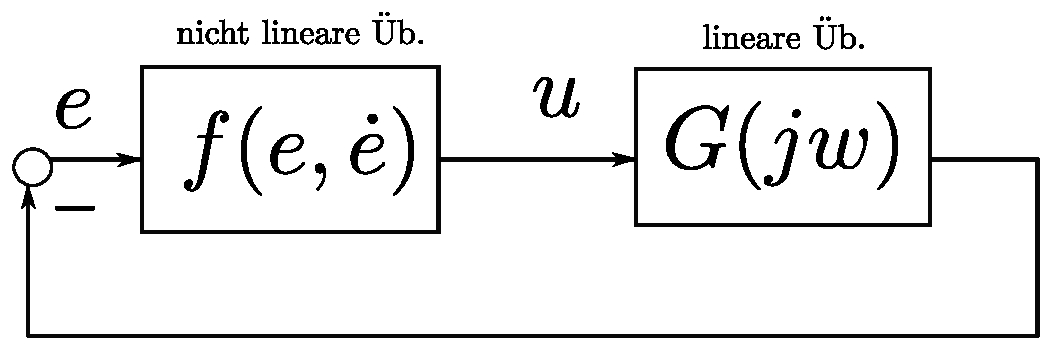
\includegraphics[width=7.5cm]{regelkr.pdf}
\end{figure}
dann geeignete Ausdruck ersetzen, so daß Beschreibung im Freqünzbereich möglich
\end{itemize}
\section{Einführungsbeispiel}
\begin{figure}[H] 
  \centering 
  \def\svgwidth{200pt} 
  %\input{Zeichnung.pdf_tex} 
  \input{regelkr1.pdf_tex} 
\end{figure} 
Annahme Dauerschwingungen vorhanden$\rightarrow $ 
\\$\quad e(t) = A \cdot \sin{(wt)}$
\\$\quad \dot{e}(t)=A\cdot w \cdot \cos(wt) $
\\$\quad w(t) = A^3 w \sin^2 (wt)\cos(wt)= A^3 w (1-\cos^2(wt))\cos(wt)$
									$     = \frac{A^3 w}{4} (\underbrace{\cos(wt)}_{\text{Grundschwingung}} -\underbrace{\cos(3 w t)}_{\text{Oberschwingung}})$
\\ Tiefpaßcharakter des lin. Übertragungsglied unterdrückt die Oberschwingung \\
mithin: \begin{equation*}w\approx \frac{A^3}{4} w\cos(wt) = \frac{A^2}{4} \frac{d}{dt} (A \sin(wt)) = \frac{A^2}{4} \frac{d}{dt}e(t)\end{equation*}
Bildbereich : $\frac{W(s)}{E(s)} = \frac{A^2}{4} s $ Übertragungsverhalten des neün Blocks, somit 
\begin{figure}[H] 
  \centering 
  \def\svgwidth{180pt} 
  %\input{Zeichnung.pdf_tex} 
  \input{regelkr2.pdf_tex} 
\end{figure} 
$w = (\underbrace{\frac{A^2}{4} jw}_{N(A,w)})(-x),\quad e(t) = A \sin(wt) \\ \Leftrightarrow e = - G(-jw)w  = -G(jw)N(A,w)\,e \Rightarrow \Big(1+G(jw) N(A,w) \Big) e = 0$ \\ $ \Leftrightarrow 1+ G(jw) N(A,w) = 0 \rightarrow 1+ (\frac{A^2}{4} jw) (\frac{\alpha}{(jw)^2 - \alpha jw +1 }) = 0$ \\ Dauerschwingung mit Amplitude $A=2 \text{ und } w=1$ 
\section{Grundlagen der Methoden}
\textit{Annahme:} es existiert eine Dauerschwingung im nichtlinearen Standartregelkreis. \\
\subsubsection{Vorraußetzung}
\begin{enumerate}
\item Lineares System
\begin{figure}[H]
\centering
\def\svgwidth{200pt} 
  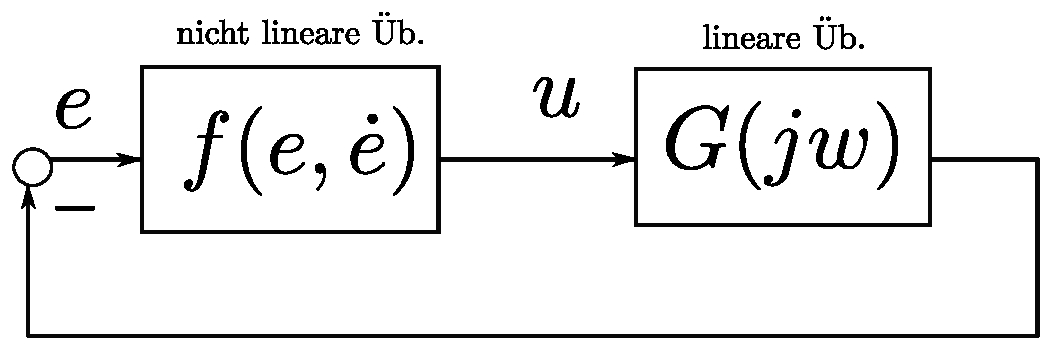
\includegraphics[width=7.5cm]{regelkr.pdf}
\end{figure}
   \begin{itemize}
 \item \textbf{L1} $G(s) = \frac{Z(s)}{N(s)} e^{-T_t s} \quad T_t > 0, \quad G(0) > 0,\quad N(s),Z(
 s) \in \mathbb{R}[s]$
 \label{L1}
\item \textbf{L2} Pole von $Z(s)/N(s) $ liegen links der $j-$Achse, 1 einfacher Pol in $s=0$
\label{L2}
erlaubt
\item\textbf{L3} $G(jw)$ hat genügend Tiefpaßcharakter  $ \text{grad}{Z} \leq \text{grad}{N} - 2$
\label{L3}
  \end{itemize}
\item Nichtlineares System
\begin{itemize}
\item \textbf{N1} $f(-e,-\dot{e}) = -f(e,\dot{e}) \\
\rightarrow $ eindeutige Kennline $\Rightarrow$ ungerade Fkt.\\
$\rightarrow$ Hysterese $\Rightarrow$ Spiegelung am Ursprung
\item \textbf{N2} $f(e)$ bzw. $f_u(e) , f_o(e) $ sind \textit{monoton steigend}!
\begin{figure}[H] 
  \centering 
  \def\svgwidth{200pt} 
    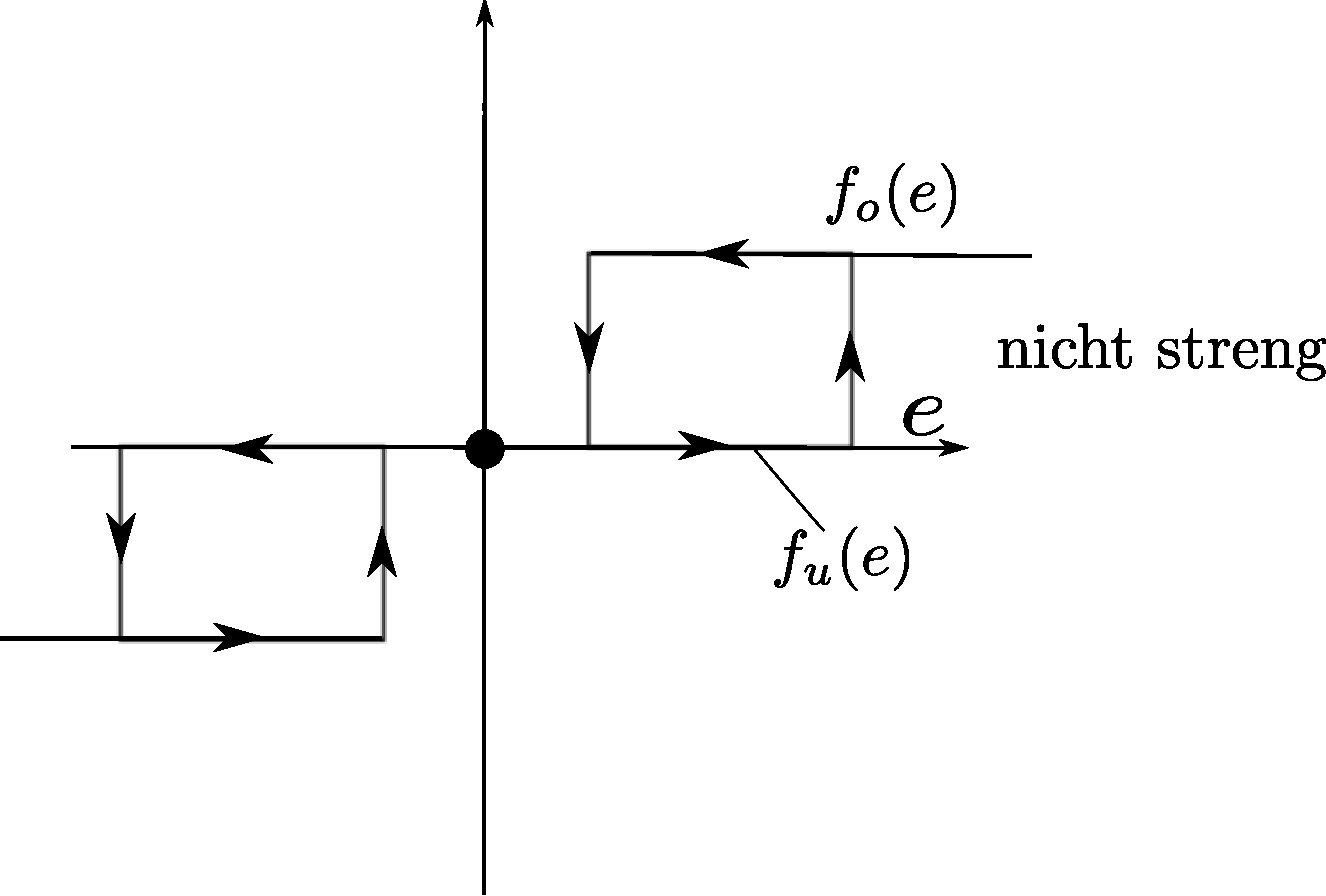
\includegraphics[width=7.5cm]{image222.pdf}
\end{figure} 
\end{itemize}
\item Die Freqünz der Dauerschwingung liegt
\begin{itemize}
\item \textbf{Z1} im Bereich der Knickfreqünzen des linearen Teilsystems
\label{Eq:Z1}
\end{itemize}
\end{enumerate}
\subsubsection{Beschreibungsfunktion}
Es gilt: $ u(t) = \frac{b_0}{2} + \sum\limits_{n=1}^{\infty} (a_n \sin{(nwt)} + b_n \cos{(nwt)})$ 
\begin{equation*}
b_0 = \frac{1}{\pi} \int\limits_{-\pi}^{\pi} u(t) \mathrm{d}(wt),\quad
a_n = \frac{1}{\pi} \int\limits_{-\pi}^{\pi} u(t) \sin{(nwt) \mathrm{d}(wt)},\quad
b_n = \frac{1}{\pi} \int\limits_{-\pi}^{\pi} u(t) \cos{(nwt) \mathrm{d}(wt)}\tag{3.1}
\end{equation*}
wegen $ b_0 = 0$ 
wenn (L3) und (Z1) erfüllt, dann können Oberschwingungen vernachläßigt werden, damit \\
$
u(t) = a_1 \sin{(wt)} + b_1 \cos{(wt)} = M \sin{(wt + \varphi)},\quad
\text{ mit } M=\sqrt{a_1^2 + b_1^2} \quad \varphi = \arctan{(\frac{b_1}{a_1})}\\
U= Me^{j(wt + \varphi)} = (a_1 + jb_1)e^{jwt} 
e(t) = A\sin{(wt)} \Rightarrow \quad E= A e^{jwt} \\
\text{Beschreibungsfunktion  } 
N(A,w) = \frac{U}{E} = \frac{a_1 +jb_1 e^{jwt}}{A e^{jwt}}\\
$ 
\begin{equation*}
\underbrace{N(A,w) = \frac{a_1 + jb_1}{A} }_{\text{Beschreibungsfunktion}}
\end{equation*}
$
A: \text{Amplitude der Dauerschwingung}\\
B: \text{Kreisfreqünz} \\
a_1, b_1 \text{ aus } (3.1)
$ 
\\
\textbf{Hinweis:} Wenn $f$ keine DGL in $e, \dot{e}$ ist, so hängt $N$ nur von $A$ ab.\\
\begin{figure}[H] 
  \centering 
  \def\svgwidth{180pt} 
  %\input{Zeichnung.pdf_tex} 
  \input{image3.pdf_tex} 
\end{figure} 
\subsubsection{Gleichung der harmonischen Balance}
Im Schwingungsgleichgewicht gilt nach $*\quad
G(jw) \cdot U = -E \text{  mit  } U = N(A,w) E \\
\Rightarrow (G(jw) N(A,w) + 1) E = 0\\
\Rightarrow G(jw)N(A,w) + 1 = 0\\
$ 
Gleichung der harm. Balance komplexe Gleichung in den Variablen $A, w$ Lösung liefert, $A,w$ der möglichen Dauerschwingung.
\section{Berechnung der Beschreibungsfunktion}
\begin{figure}[htbp]
\begin{minipage}[c]{8.0cm}
\def\svgwidth{180pt} 
 \input{image4.pdf_tex} 
\end{minipage}
\begin{minipage}[c]{7cm}

\begin{tabular}{lll}
Es gilt: &&\\
$a_1 = \frac{1}{\pi} \int\limits_{0}^{2\pi} u(t) \sin{(wt)} \mathrm{d}(wt)$ &&\\
$a_1 = \frac{2}{\pi} \int\limits_{0}^{\pi} u(t) \sin{(wt)} \mathrm{d}(wt)$ &&\\
$a_1 = \frac{2}{\pi} \int\limits_{\varphi_1}^{\varphi_2}  = b\sin{(wt)} \mathrm{d}(wt) = \frac{2b}{\pi} (\cos{\varphi_1} - \cos{\varphi_2})$&&\\
analog:
$b_1 = \frac{2b}{\pi}\Big[ \sin{(\varphi_2)} - \sin{(\varphi_1)}\Big]$ &&\\
$\text{Bestimmung } \varphi_1, \varphi_2, \quad A\sin{\varphi_1} = a \leftrightarrow \varphi_1 = \arcsin{\frac{a}{A}} $&&\\
$\cos{\varphi_1} = +\sqrt{1 - \sin^2{\varphi_1}} $&&\\
$\cos{\varphi_1} = \sqrt{1 - (\frac{a}{A})^2}$ &&\\
$A\sin{\varphi_2} = q a > \frac{\pi}{2}$&&\\
$\cos{\varphi_2} = - \sqrt{1- (\frac{qa}{A})^2}$&&\\
$\text{mithin: }$&&\\
$a_1 = \frac{2b}{\pi} \left(  \sqrt{1- (\frac{a}{A})^2} + \sqrt{1- (\frac{qa}{A})^2}   \right)$&&\\
$b_1 = \frac{2b}{\pi} \left(  \frac{qa}{A} - \frac{a}{A}\right) = \frac{2ba}{\pi A} (q-1)$&&\\
$\underbrace{N(A) = \frac{a_1 + jb_1}{A}}_{\text{Dreipunktglied mit Hysterese}}$&&
\end{tabular}
\end{minipage}
\end{figure} 
Spezialfälle
\begin{itemize}
\item $q=1$ Dreipunktglied ohne Hysterese\\
$ N(A) = \frac{4b}{\pi A} \sqrt{ 1- (\frac{a}{A})^2} \quad A>a $
\item $q=1, a=0 \Rightarrow$ Zweipunktglied ohne Hysterese\\
$N(A) = \frac{4b}{\pi A} \quad A>0 $
\item $q=-1$ Zweipunktglied mit Hysterese \\
$N(A) = \frac{4b}{\pi A} = \sqrt{ 1 - (\frac{a}{A})^2 } - j \frac{4ab}{\pi A^2} $\\
Allgemein: wenn keine Hysterese, dann Imaginäranteil $(b_1)$ Null!
\end{itemize}
\section{Lösung der Gleichung der harmonischen Balance}
\begin{figure}[htbp]
\begin{minipage}[c]{9.0cm}
\def\svgwidth{250pt} 
\input{image6.pdf_tex} 
\end{minipage}
\begin{minipage}[c]{7cm}

\begin{tabular}{lll}
$G(jw) + N(A,w) +1 = 0$&&\\
analytisch:&&\\
$N(A,w) = -\frac{1}{G(jw)} \Rightarrow \operatorname{Re}(N(A,w)) = \operatorname{Re}(-\frac{1}{G(jw)})$ &&\\
$\operatorname{Re}(N(A,w)) = \operatorname{Re}(-\frac{1}{G(jw)})$&&\\
graphisch in der komplexen Zahlenebene &&\\
$\underbrace{G(jw) = -\frac{1}{N(A,w)}}_{\text{negative inverse Beschreibungsfunktion}}$&&\\
&&\\
Dauerschwingungen? &&\\
$\mathrm{Im}(G(jw_0)) = 0 $ &&\\
$\operatorname{Re}(G(jw_0)) < -a$ \\
\end{tabular}
\end{minipage}
\end{figure} 
\section{Stabilität von Dauerschwingungen}
\begin{figure}[H] 
  \centering 
  \def\svgwidth{120pt} 
  %\input{Zeichnung.pdf_tex} 
  \input{image7.pdf_tex} 
\end{figure} 
$k: \quad N(A)$
\begin{itemize}
\item $A= A_p \rightarrow$ Dauerschwingung $\rightarrow \begin{matrix} N(A_p)& = & K_p \\G(jw) & =& -\frac{1}{K_p} \end{matrix}\\
A = A_p + \Delta A \text{  keine Dauerschwingung mehr}\\
K = N(A_p + \Delta A)$ 
\begin{figure}[H] 
  \centering 
  \def\svgwidth{350pt} 
  %\input{Zeichnung.pdf_tex} 
  \input{image8.pdf_tex} 
\end{figure} 
\end{itemize}
\chapter{Stabilität nach Ljapunov}
bisher behandelt:
\begin{itemize}
\item Systeme 2. Ordnung
\item Verhalten von Systemen höherer Ordnung schwer zu beurteilen
\item Linearisierung von Ruhelagen Aussagen in Umgebung
\end{itemize}
Ljapunov-Theorie:
\begin{itemize}
\item Untersuchung der Stabilität von Ruhelagen, ohne die Trajektorie (Lösung) zu kennen
\begin{enumerate}
\item indirekte Methode (Linearisierung)
\item direkte Methode
\end{enumerate}
\end{itemize}
\section{Stabilitätsbegriff}
Wir betrachten autonomes System der Form: \begin{equation}\dot x = f(x)\tag{4.1}
\label{EQ:4.1}
\end{equation}
\begin{equation*}
f: \mathbb{R}^n \rightarrow \mathbb{R}^n, x(0) = x_0 \in \mathbb{R}^n \text{ Anfangswert}
\end{equation*}
$\phi_t(x) \dots $ Fluss von (\ref{EQ:4.1})), d.h. allgemeine Lösung
\\Ruhelage $x^e \in \mathbb{R}^n \qquad 
\dot x = 0 \underbrace{\Leftrightarrow}_{(\ref{EQ:4.1})} f(x^e)= 0 \Leftrightarrow \phi_t(x^e)=x^e
$\\
Annahme (ohne Einschränkung): $x^e=0$\\
(wenn $x^e \ne 0, $ : Koordinatentransformation $\tilde x = x- x^e \Rightarrow \tilde x^e = 0 $)
\\
\begin{itemize}
\item \textbf{Definition 4.1:} Die Ruhelage $x^e = 0$ von (\ref{EQ:4.1})) heisst stabil (im Sinne von Ljapunov), wenn zu jedem $\varepsilon > 0$ ein $\delta (\varepsilon) > 0$ existiert, so dass
\begin{equation*}
||x_0|| < \delta \Rightarrow ||\phi_t(x_0)||< \varepsilon \quad \forall t \ge 0.
\end{equation*}
\begin{figure}[H] 
  \centering 
  \def\svgwidth{350pt} 
  %\input{Zeichnung.pdf_tex} 
  \input{im1.pdf_tex} 
\end{figure} 
\begin{itemize}
\item Anschaulich: Wenn die Trajektorie $\phi_t(x_0)$ die Umgebung mit dem \textit{Radius} $\varepsilon$ nicht verlassen soll, so muss man nahe genug an der Ruhelage $x^0 = 0 $ starten, nähmlich in einer Umgebung mit Radius $\delta$. 
\item Bemerkung: 
Instabilität heisst hier nicht , dass die Trajektorie über alle Grenzen wächst,
\item Stabilität heisst hier nicht, dass die Trajektorie gegen einem Punkt konvergiert bzw. einläuft.
\end{itemize}
\item \textbf{Definition 4.2:} Die Ruhelage $x^0 = 0$ von (\ref{EQ:4.1}))heisst, attraktiv/anziehend, wenn es eine Zahl $\delta > 0$ gibt, so dass
\begin{equation*}
||x_0|| < \delta \Rightarrow \lim \limits_{t\rightarrow \infty} \phi_t(x_0) = 0.
\end{equation*}
\item \textbf{Definition 4.3:} Ist die Ruhelage $x^e = 0$ von \ref{EQ:4.1} stabil und anziehend, dann nennt man sie \textit{asymptotisch stabil}.
\begin{itemize}
\item Hinweis: Eine anziehende Ruhelage muss nicht notwendigerweise stabil i.s. \textit{Ljapunov} sein.
\end{itemize}
\subitem Problem bei Definition 4.3: Keine Zeitaussage wie schnell konvergiert das?
\item \textbf{Definition 4.4: } Die Ruhelage $x^e = 0$ von (\ref{EQ:4.1})) heisst \textit{exponentiell stabil }, wenn gilt 
\begin{equation*}
\exists \, \alpha, \lambda > 0,\quad \forall t\ge 0: \underbrace{ || \phi_t(x_0) ||}_{x(t)} \le \alpha \underbrace{|| x_0 || }_{x(0)} e^{-\lambda t}
\end{equation*}
in einer Umgebung $B$ im den Ursprung.
\begin{itemize}
\item Anschaulich: Trajektorie konvergiert mindestens so schnell gegen Ursprung wie eine Exponentialfunktion
\item Es gilt: Exponentialstabilität $ \stackrel{\nLeftarrow}{\Rightarrow} $ Asymptotischstabilität
\item Beispiel: $\dot x  = -(1+ \sin^2(x)) x\\
\Rightarrow x(t) = x(0) \cdot \exp\Big({ \int \limits_{0}^{t} \underbrace{(1+\sin^2x(\tau))}_{\ge 1}d\tau }\Big)\\
\Rightarrow |x(t)| \le x(0)e^{-t} \\
\Rightarrow x^e = 0
$ ist exponentiellstabil\\
Bisher nur lokale Aussagen
\end{itemize}
\item \textbf{Definition 4.5:} Wenn die Eigenschaften der asympt./exp.Stabilität eine Ruhelage für alle Anfangsbedingungen (= auf ganz $\mathbb{R}$) gilt, so heisst die Ruhelage \textit{gloabl asympt./exp stabil.}
\begin{itemize}
\item Hinweis: 
\begin{enumerate}
\item linear: lokal $=$ global
\item nichtlinear: global eher selten
\item asympt. : nur, wenn es genau 1 Ruhelage gibt 
\begin{figure}[H] 
  \centering 
  \def\svgwidth{350pt} 
  %\input{Zeichnung.pdf_tex} 
  \input{im2.pdf_tex} 
\end{figure} 
\end{enumerate}
\end{itemize}
\end{itemize}
\section{Direkte (zweite) Methode von Ljapunov}
\begin{itemize}
\item Ziel: \\Stabilitätsaussage , ohne Trajektorie (Lösung) zu kennen.
\item Grundidee: 
\begin{itemize}
\item Wenn Gesammtenergie eins mechan. elektr. chem. kontinuierlich abnimmt, dann muss das System zur Ruhelage kommen
\item Gesammtenergie: Skalar
\end{itemize}
\end{itemize}
\subsection{Einführungsbeispiel}
\begin{figure}[H] 
  \centering 
  \def\svgwidth{250pt} 
  %\input{Zeichnung.pdf_tex} 
  \input{im3.pdf_tex} 
\end{figure} 
\begin{equation*}
\begin{matrix}
u_c = u - R\cdot i_R - L \frac{d\,i_R}{d\,t}&& G(u_c)> 0\\
i_R = G\,u_c + C \frac{d\,u_c}{d\,t} && R(i_R) > 0\\
\dot u_c = \frac{1}{C}(-G u_c + i_R) && C(u_c) >0\\
\dot i_R = \frac{1}{L} (-u_c - R\, i_R + U) && L(i_R)> 0 \\
&& \\
\end{matrix}
\end{equation*}
Kurzschluss : $U=0$\\
Energie: 
\begin{align*}
V = &\,\frac{1}{2} C u_c^2 + \frac{1}{2} L \, i_R^2\\
\dot V =& \,C u_c \cdot \dot u_c + L i_R \dot i_R \\
=&\, u_c (-G u_c + i_R) + i_R (-U_L -R i_R)\\
=& -G u_c^2 + i_R u_c - i_R u_c - R i_R^2\\
=& -G \,u_c^2 - R\,i_R^2 < 0 \text{  für } (u_c, i_R) \ne (0,0)
\end{align*}
$\Rightarrow $Energei wird kontinuierlich abgebaut!\\
Verallgemeinerung: Ljapunov-Methode
\subsection{Positiv Definite Funktionen}
\begin{itemize}
\item \textbf{Definition 4.5:} Sei $D \le \mathbb{R}^n $ eine offene Umgeb. von 0.\\
Eine Funktion $V: D\rightarrow \mathbb{R}$ heisst \textit{lokal positiv definit} wenn
\begin{enumerate}
\item $V(x) $ ist stetig differenzierbar
\item $V(0)$ 
\item $V(x)> 0$ für alle $x \in D {0} $ gilt zusätztlich $D = \mathbb{R}^n $ und $\exists d> 0$ und $inf\quad V(x) > 0 $, dann heisst $V$ \textit{positiv definit} $ ||x|| > d$

Genügt $V$ in 3. lediglich der Bed.\\
\item [3'] $V(x) \ge 0 \quad \forall \, x\in D {0} $ dann heisst $V$ \textit{(lokal) positiv semidefinit}
\end{enumerate} 
$V(x)$ heisst (lokal ) negativ (semi-) definit, wenn \textit{ $V(x)$} (lokal) positiv (semi) definit!
\item Beispiel: 
\begin{itemize}
\item $V(x)$ aus Abschnitt 4.2.1 ist positiv definit
\item mechanische Energie eines Fadenpendels 
\begin{figure}[H] 
  \centering 
  \def\svgwidth{300pt} 
  %\input{Zeichnung.pdf_tex} 
  \input{im4.pdf_tex} 
\end{figure} 
$V(x, \dot x) = \frac{1}{2} m l^2 \dot x^2 + m g l (1-\cos(x))$ positiv definit
\item kinetische Energie des Fadenpendels: \\$
V^* (x, \dot x) = \frac{1}{2} ml^2 \dot x^2 \ge 0\\
$
nur positiv semidefinit: $V(x, \dot x) = 0 \text{ für } \dot x = 0, x\ne 0$
\item $V(x_1,x_2,x_3) = (x_1 + x_2)^2$ positiv semidefinit
\item $V(x_1, x_2,x_3) = x_1 - 2x_2 + x_3^2$ nicht positiv semidefinit $\Rightarrow$ nicht pos. definit
\end{itemize}
\end{itemize}
\subsection{Stabilitätskriterium}
\begin{itemize}
\item Satz 4.1: Sei $x^e = 0$ eine Ruhelage von (4.1) und $D \in \mathbb{R}^n $ eine offene Umgebung von $0$. Existiert eine Funktion $D\rightarrow \mathbb{R}$ derart, dass

\begin{itemize}
\item $V(x)$ ist auf $D$ positiv definit L
\item $\dot V(x)$ ist auf $D$ negativ semidefinit
\end{itemize} 

dann ist $x^e = 0$ lokal stabil \\
ist $\dot V(x)$ auf $D$ sogar negtativ definit , dann ist $x^e$ lokal asymptotisch stabil. \\
Zu dem Fall heisst $V$ Ljapunov Funktion
\item Hinweis: $\dot V(x) = \mathbb{L}_fV(x) $ ist Lie-Ableitung von $V$ entlang des Vektorfeldes $f$
\item Vorgehen: Konstruiere zu einem System (4.1) eine Funktion $V(x)$ und zeige, dass es sich um eine Ljapunov-Funktion handelt.
\item Achtung: Kriterium ist nur hinreichend (wenn $V(x)$ keine Ljapunov-Funktion, dann folgt daraus nicht, das $x_e = 0$ instabil!)
\begin{itemize}
\item Beispiel: $\dot x = - g(x) $
\begin{itemize}
\item $g(x)$ lokal Lipschitz auf (-a,a)
\item $g(0) = 0$ img1 $xg(x) > 0 \quad \forall x\ne 0 \land x\in (-a,a)\\
V(x) = \int\limits_{0}^{x} g(\xi)d\xi \rightarrow\text{ positiv definit}\\
\dot V(x) = \mathbb{L}_g V(x) = \frac{\partial V}{\partial x} \dot x = \frac{\partial V}{\partial x}(-g(x))= -g^2(x)< 0 \forall x\ne 0\rightarrow$ negativ definit $x_e = 0$ lokal asymptotisch stabil.
\item Beispiel: $
\begin{pmatrix}
\dot x_1 &= & x_2\\
\dot x_2 &=& -a\sin(x_1) - b x_2 
\end{pmatrix}\qquad a,b>0\\
$ Fadenpendel mit Reibung , $a = \frac{g}{l}, b:\text{Reibung }$\\
Ljapunov-Funktion Kandidat\\ $ V(x) = a (1- \cos(x_1)) + \frac{1}{2} x_2^2 \rightarrow$ positiv definit\\
$\dot V(x) = a\sin(x_1)\dot x_1 + x_2 \dot x_2 = a x_2 \sin(x_1) - a x_2 \sin(x_1) - b x_2^2\\
\dot V(x) = -bx_2^2$ negativ semidefinit $\dot V(x) = 0 \Leftrightarrow x_2 = 0 \land x_1 \in \mathbb{R}$ 
img2 negativ semidefinit (nur Stabilität nachgewiesen!)
\end{itemize} 
\end{itemize}
\item \textbf{Definition:} Sei $x_e = 0$ eine asymptotisch stabile Ruhelage von (4.1). Man nennt die \\
Menge $B = \left\{ x_0 \in \mathrm{R}^n | \lim_{t \to \infty} \phi_t(x_0) = 0 \right\}$ den Einzugsbereich von $x_e$ img3\\
Ist $B = \mathbb{R}^n $, so ist die Ruhelage global asymptotisch stabil\\
\item \textbf{Definition:} Eine Menge $M \in \mathbb{R}^n $ heisst positiv invariante Menge des Systems $\dot x = f(x)$, wenn das Bild der Menge $M$ under dem Fluss $\phi_t$ die Menge $M$ selbst ist, d.h.\\ $\phi_t(M) = M\, \forall \, t>0$ \\
img4 alles,was in $M$ startet, (oder in $M$ hineinläuft), verbleibt in $M$ 
\item \textbf{Satz 4.2:} Sei $x_e = 0$ eine Ruhelage von (4.1). Existiert eine Funktion $V :\mathbb{R}^n \rightarrow \mathbb{R}$ mit 
\begin{itemize}
\item $V(x) $ positiv definit (global)
\item $\dot V(x)$ negativ definit (global)
\item $V(x)$ radial unbeschränkt $\rightarrow \lim_{\|x\| \to 0} V(x) \rightarrow \infty$\\
Dann ist $x_e = 0$ global asymptotisch stabil.
\end{itemize}
\item \textbf{Satz 4.3:} Sei $x_e = 0$ Ruhelage des Sysems (4.1) und $V: D\rightarrow \mathbb{R}$ wenn
\begin{itemize}
\item $V(x_e) = 0$
\item $V(x) > 0 $ für $\|x\| $ klein
\item $\dot V(x) $ lokal positiv definit ist dann ist $x_e $ instabil
\end{itemize}
\end{itemize}
\section{Invarianzprinzip (Satz von La Salle)}
\begin{itemize}
\item Problem: Direkte Methode von Ljapuvon weist häufig nur Stabilität, aber keine asymptotische Stabilität nach (wenn $\dot V(x)$ nur negativ semidefinit)
\item \textbf{Satz 4.4:} für ein System des Typs (4.1) sei eine Funktion $V: \mathbb{R}^n \rightarrow \mathbb{R}$ gegeben
\begin{itemize}
\item Für ein $l > 0$ ist $\Omega_e = \{ x\in \mathbb{R}^n | V(x) \le l \}$ kompakt (abgeschlossen/beschränkt)
\item $\forall x \in \Omega_e$ gilt $\dot V(x) \le 0$
\item $R = \{ x\in \Omega_e | \dot V(x) = 0\}$
\item grösste positiv invariante Menge $M$ in $R$ bestimmen\\
$\Rightarrow$ dann strebt für $t\to \infty$ jede Trajektorie, die in $\Omega_e$ startet, gegen $M$ \\wenn $M= x_e$ dann ist $x_e$ lokal asymptotisch stabil img5
\begin{align}
\dot x_1 =& x_2\tag{a}\\
\dot x_2 =& -a \sin(x_1) - bx_2\tag{b}\\
R = &\{ x\in \Omega_e | x_2 = 0\}\notag\\
\end{align}
$ 
x_2 \equiv 0 \underbrace{\Rightarrow}_{(a)} \dot x_1 = 0 \quad \dot x_2 = 0\\
(b) \Rightarrow  x_1 = 0 \Rightarrow M = (0,0) = x_e \qquad x_e = 0 \text{ lokal asymptotisch stabil }
$
\end{itemize}
\end{itemize}
\section{Variable Gradientenmethode}
\begin{itemize}
\item Ziel: Systematische Konstruktion einer Ljapunov-Funktion.
\item Beispiel: 
\begin{align}
\dot x_1 = & x_2 \tag{(4.3) Ruhelage $x_e = (0,0)$}\\
\dot x_2 = & - x_2 - x_1^3 
\end{align}
Vorgabe eines Gradienten für skalare Funktion $V(x)$\\
$(\frac{\partial V}{\partial \underline x})^T = 
\begin{pmatrix}
\frac{\partial V}{\partial x_1}\\
\frac{\partial V}{\partial x_2}
\end{pmatrix} = 
\begin{pmatrix}
V_{11}(\underline x) x_1 + V_{12}(\underline x) x_2\\
V_{21}(\underline x) x_1 + V_{22}(\underline x) x_2
\end{pmatrix}
\quad $Integrabilitätsbedingungen müssen erfüllt sein\\
$ 
\frac{\partial}{\partial x_i} \frac{\partial V}{\partial x_j} = \frac{\partial }{\partial x_j} \frac{\partial V}{\partial x_i} \quad i \ne j$ 
\item Erinnerung: Ist $(\frac{\partial V}{\partial \underline x})^T$ ein Gradient von $V(\underline x)$ so ist das Integral über $(\frac{\partial V}{\partial \underline x})^T$ wegunabhängig \\
Für (4.3) lauten Integrabilitätsbedingung \\
$\frac{\partial}{\partial x_2} = (V_{11}(\underline x) x_1 + V_{12}(\underline x) x_2) = \frac{\partial }{\partial x_1} (V_{21}(\underline x) x_1 + V_{22}(\underline x) x_2)\\
\frac{V_{11}(\underline x)}{\partial x_2} x_1 = \underbrace{\frac{\partial V_{12}(\underline x)}{\partial x_2} }_{= 0} x_2 + V_{12}(\underline x) = \underbrace{ \frac{\partial V_{21}(\underline x)}{\partial x_1} }_{=0} x_1 + V_{21} (\underline x) + \frac{\partial V_{22}(\underline x)}{\partial x_1} x_2
$
\item Wahl: $\left.
\begin{matrix}
V_{12}(\underline x) &= & V_{21} (\underline x) = b\\
V_{11}(\underline x) &=& a(x_1)\\
V_{22}(\underline x) &=& c (x_2)
\end{matrix}\right\} \Rightarrow \frac{\partial V}{\partial \underline x} = 
\begin{pmatrix}
a(x_1) x_1 + b x_2\\
b x_1 + c(x_2) x_2
\end{pmatrix}
$ \\
Festlegung von $a(x_1), c(x_2) $ und $b$, so dass $\dot V$ negativ definit \\
$
\dot V = \frac{\partial V}{\partial x_1}\dot x_1 + \frac{\partial V}{\partial x_2} \dot x_2 = -b x_1^4 + (b-c(x_2))x_2^2 + \underbrace{(a (x_1)- b - c(x_2) x_1^2) x_1 x_2 }_{term0}\\
\quad$ muss negativ definit sein!\\
$\begin{matrix}
a(x_1) &=& b + c(x_2) x_1^2\\
c(x_2) &=& d
\end{matrix} \qquad $
damit $term0$ = 0\\
\item liefert: $\dot V = -b x_1^4 + \underbrace{(b-d)}_{term1} x_2^2$\\
\item Wahl: $d> b \rightarrow $ damit $term1 < 0$ negativ definit \\
Bestimmung von V Integration von $(\frac{\partial V}{\partial \underline x})^T$ über $x_1 , x_2$ da wegunabhängig \\$
V(x) = \int \limits_{0}^{x_1} \frac{\partial V}{\partial x_1} (\xi , 0) + \int\limits_{0}^{x_2} \frac{\partial V}{\partial x_2} (x_1, \xi)d\xi
$

\begin{align*}V(x) = &\frac{d}{4} x_1^2 + \frac{b}{2} x_1^2 + b x_1 x_2 + \frac{d}{2} x_2^2 \text{   muss positiv definit sein! }\\
 = &\frac{b}{2} (x_1^2 + 2 x_1 x_2 + x_2^2) - \frac{b}{2}x_2^2 + \frac{d}{2}x_2^2\\
= &\frac{d}{2} (x_1 + x_2)^2  + (\frac{d}{2}- \frac{b}{2})x_2^2
\end{align*}\quad positiv deinit für $b> 0 $ und $d>b$
\end{itemize}
\chapter*{\textbf{B:} Regelung nichtlinearer Systeme}
\section*{\textbf{B.1:} Stabilisierungsprobleme}
\begin{itemize}
\item Asymptotische Stabilisierung\\
Nichtlinearer System: $\dot x = f(x,u,t) $ \\Regelgesetz finden $u = g(\cdot ,t)$ so dass wenn $x_0 \in \Omega, \quad \phi_t(x_0) \rightarrow 0$ für $t\to \infty$\\
$u = g(x,t) \rightarrow $ statisches Regelgesetz $\dot u = g(u,x,\dot x,t) \rightarrow $ dynamisches Regelgesetz \\
wenn $\phi_t(x_0) \rightarrow x_d$ gewünscht, dann Transformation $x^* = x-x_d$
\item Folgeregelungsproblem\\
System: $\dot x = f(x,u,t) \quad y= h(x) $\\
Solltrajektorie für $y: y_d(t)$\\
Regelgesetz $u = g(\cdot , t) ,$ so dass,wenn $x_0 \in \Omega \quad y(t) - y_d(t) \rightarrow 0 $ für $t\to \infty$ und $x$ beschränkt.
\end{itemize}
\section*{\textbf{B.2: }Einführungbeispiel}
System: \begin{align*}\dot x =& ax - bx^3 + u \quad &a,b>0\\
y=&x &x,u \in \mathbb{R}
\end{align*}
Regelgesetz $1$ Wunsch $u$ so dass geschlossene Kreis folgender Dynamik genügt
\begin{align*}
\dot x = - k x\quad k>0
\end{align*}
Wahl: 
\begin{align*}
u =& - a x + b x^3-kx \quad &\text{Reglerparameter: k}\\
u=& - (k+a)x + b x^3 &k>0
\end{align*}
Regelgesetz kompensiert auch den Term $-bx^3$.\\
Sinnvoll? Nein, denn $-bx^3$ ist eine nichtlineare Dämpfung, die dafür sorgt dass $x$ stets beschränkt ist, auch wenn $ax$ für Instabilität sorgt.\\
Folgendes Regelgesetz 2 reicht\\
$u = - (k+a)x \quad \rightarrow \dot x =-kx - bx^3 \quad x=0 $ asymptotisch stabil

\begin{center}
  \begin{tabular}{ l | c | r }
     & +Vorteil & -Nachteil \\ \hline
    Regelgesetz 1 & exponentielle Stabilisierung & Implementierungsaufwand \\ \hline
   Regelgesetz 2 & Einfachheit & nur asymptotisch Stabilisierung \\
    \hline
  \end{tabular}
\end{center}
\section*{\textbf{B.3: } Vorsteuerung}
In nichtlinearer Regelungsaufgaben ist die Vorsteuerung häufig wichtig
\begin{itemize}
\item liefert Information für Überführungsaufgaben
\item kompensiert bekannte Störungen\\
Bild1. Regler kompensiert nur Fehler in der Steuerung und Störungen Bild2
\end{itemize}
\chapter{Intergrator-Backstepping}
\section{Einführungsbeispiel}
System: \begin{align}\dot x_1 =& x_1^2 - x_1^3 + x_2 \tag{5.3a}\\
\dot x_2 = & u \tag{5.3b}
\end{align}
\begin{itemize}
\item Schritt 1: Stabilisierung des $1.$ Teilsystems\\
$\dot x_1 = x_1^2 - x_1^3 + \underbrace{x_2}_{ = \alpha(x_1)} \rightarrow$ Betrachtung als neuer Eingang mit dem Regelgesetz $x_2 = \alpha(x_1)$
\begin{align}
\rightarrow \dot x_1 = x_1^2 - x_1^3 + \alpha(x_1) \tag{5.4}
\end{align}
sinnvolle Wahl (vergl. Abschnitt \textbf{B.2})\\
$\alpha(x_1) = -x_1^2 - k_1x_1 \qquad k_1 > 0$\\
Damit Dynamik  geschlossenen Kreises des $1.$ Teilsystems: $\dot x_1 = -x_1^3 - k_1x_1$\\
Stabil? \begin{align*}V_1(x_1) =& \frac{1}{2} x_1^2 \text{ positiv definit radial unschränkt}\\
V_1(x_1) = & \frac{1}{2} x_1^2 \\
\dot V_1(x_1) =& x_1\dot x_1 = -x_1^4 - k_1 x_1^2 \text{ negativ definit } 
\end{align*}
ja global asymptotisch stabil
\item Schritt 2: Fehler in $\alpha(x_1)$\\
$\rightarrow x_2$ muss sich so verhalten , wie durch $\alpha(x_1)$ gefordert. Real ergibt sich jedoch Fehler: \begin{align*}z_2:= &x_2 - \alpha(x_1)\\
=& x_2 + x_1^2 + k_1 x_1
\end{align*} 
$z_2 $ muss gegen Null gehen, damit $x_2 = \alpha(x_1)$ erfüllt und somit auch $x_1 \to 0$ geht. Also wird Differentialgleichung für $z_2$ benötigt 
\begin{align*}
\dot z_2 = &\dot x_2 + 2x_1 \dot x_1 + k_1 \dot x_1\\
=&\underbrace{\dot x_2}_{5.3b} + (2 x_1 + k_1) \underbrace{\dot x_1}_{5.3a}\\
\dot z_2 = & u + (2x_1 + k_1)(x_1^2 - x_1^3 + \overbrace{z_2 + \alpha(x_1)}^{= x_2}) \\
\text{ System in neuen Koordinaten }\\
\dot x_1 = & x_1^2 - x_1^3 + z_2 - \underbrace{x_1^2 - k_1 x}_{\alpha(x_1)}\\
\dot x_1 = & -x_1^3 - k_1x_1 + z_2 \tag{5.5a}\\
\dot z_2 = & u + (2 x_1 + k_1) (-x_1^3 - k_1 x_1 + z_2) \tag{5.5b}\\
\end{align*}
\item Schritt 3: Wie $u$ wählen , damit $z_2 \to 0$
\begin{align*}
V_2(x_1,z_2) = &V_1(x_1) + \frac{1}{2} z_2^2\\
\dot V_2(x_1,z_2) = & x_1 \dot x_1 + z_2 \dot z_2 = \underbrace{- x_1^4 - k_1x_1^2 + x_1 z_2 + z_2 (u +(2x_1 + k_1)(-x_1^3 - k_1 x_1 + z_2))}_{\rightarrow \text{ muss negativ definit sein }\to u!}\\
\end{align*}
$\dot V_2 $ ist zum Beispiel wie folgt negativ definit \\
$\dot V_2(x_1,z_2) = - x_1^4 - k_1 x_1^2 - \underbrace{k_2 z_2^2}_{u \text{ so wählen,dass das gilt}} \qquad k_1,k_2 > 0 \\
u = -k_2z_2 - (2x_1 + k_1)(-x_1^3 - k_1 x_1 + z_2) - x_1\\
\rightarrow$ Regelgesetz mit $z_2 = x_2 + x_1^2 + k_1 x_1$ und Parameter $k_1, k_2 > 0$
\end{itemize}
\section{Verallgemeinerung}
Systemklasse
\begin{align*}
\underline{\dot x_1} = & \underline{f}(\underline{x_1}) + \underline{g}(\underline{x_1})x_2\\
\dot x_2 = & u\\
\underline x_1 &\in \mathbb{R}^n\\
x_2 &\in \mathbb{R}, u \in \mathbb{R}
\end{align*}
\begin{itemize}
\item Schritt 1: Stabilisierung 1.Teilsystem $x_2 = \alpha(\underline x_1)$ \textit{ fiktives Regelgezetz }\\ $\underline {\dot x_1} = \underline f (\underline x_1) + \underline g(\underline x_1) \alpha (\underline x_1)$ \\
Ruhelage $\underline x_1 = 0 $ ist zu stabilisieren $\Rightarrow \alpha(\underline x_1)$ entsprechend wählen. \\
Ljapunov-Funktion $V(\underline x_1) $ positiv definit \\
üblicherweise: 
\begin{align*}
V(\underline x_1) = &\frac{1}{2} x_{11}^2 + \dots + \frac{1}{2} x_{1n}^2\\
\dot V(\underline x_1) = & \frac{\partial}{\partial \underline x_1} V(\underline x_1) (\underline f(\underline x_1) + \underline g(\underline x_1) \alpha (\underline x_1))\\
\end{align*}
$\alpha(\underline x_1)$ so, dass gilt $\dot V(\underline x_1) \le W(\underline x_1) \le 0$
\item Schritt 2: Fehler zwischen $x_2$ und $\alpha (\underline x_1)$\\
Fehler: $z_2 = x_2 - \alpha (\underline x_1) \rightarrow$ neue Koordinate\\
alte Koordinaten. $(\underline x_1, x_2)$\\
neue Koordinaten. $(\underline x_1, z_2)$\\
Stabilisieren : 
\begin{align*}
\underline x_1 = &0 \\
z_2 = &0
\end{align*} siehe oben damit Fehler zwischen $x_2$ und $\alpha(\underline x_1) = 0$\\
System in neuen Koordinaten\\
\begin{align*}
\underline {\dot x_1} =& \underline f(\underline x_1) + \underline g(\underline x_1) (z_2 + \alpha(\underline x_1))\\
\dot z_2 = & \dot x_2 - \dot \alpha(\underline x_1)\\
=& u - \frac{\partial \alpha(\underline x_1)}{\partial \underline x_1} (f(\underline x_1) + \underline g(\underline x_1)(z_2 + \alpha(\underline x_1)) )
\end{align*}
\item Schritt 3: Wahl von $ u $ so, dass auch $z_2 = 0$ asymptotisch stabil.\\ $V_2(\underline x_1,z_2) = V_1(\underline x_1) + \frac{1}{2}z_2^2$ positiv definit, radial unbeschränkt\\
\begin{align*}
\dot V_2(\underline x_1, z_2) =& \frac{\partial V_1}{\partial \underline x_1} \underline{\dot x_1} + z_2 \dot z_2\\
=& \frac{\partial V_1}{\partial \underline x_1} \left(\underline f(\underline x_1)+ \underline g(\underline x_1)(z_2 + \alpha(\underline x_1)) \right) + z_2\left(u -\frac{\partial \alpha(\underline x_1)}{\partial \underline x_1} (\underline f(\underline x_1) + \underline g(\underline x_1)(z_2 + \alpha(\underline x_1) ) ) \right)\\
=& \underbrace{\frac{\partial V_1}{\partial x_1}(\underline f(\underline x_1) + \underline g(\underline x_1)\alpha(\underline x_1) ) }_{\le W_1(\underline x_1) \text{ negativ definit }} + \underbrace{\frac{\partial V_1}{\partial \underline x_1}\underline g(\underline x_1) z_2 + z_2\left(u - \frac{\partial \alpha(\underline x_1)}{\partial \underline x_1} (\underline f(\underline x_1) + \underline g(\underline x_1))(z_2 + \alpha(\underline x_1) ) \right) }_{\text{ negativ definit machen über Wahl von $u$ }}
\end{align*}
$u \rightarrow $ so, dass $\dot V_2$ negativ definit \\fehlt etwas hier
\end{itemize}
Anmerkungen: 
\begin{enumerate}[a)]
\item Systeme des Typs
\begin{align*} 
\underline x_1 \in \mathbb{R}^n\\
x_2, u \in \mathbb{R}\\\\
\dot{\underline x_1} =&\underline f(\underline x_1) + \underline g(\underline x_1)x_2\\
\dot x_2 =& f_2(\underline x_1,x_2) + \underline g_2(\underline x_1,x_2)u
\end{align*} Wahl eines neuen Eingangs $u^*$ mit $u^* = \frac{1}{g_2(\underline x_1,x_2)} (u - f_2(\underline x_1, x_2))$\\
führt auf 
\begin{align*}
\underline{\dot x_1} = & \underline f(\underline x_1) + \underline g(\underline x_1)x_2\\
\dot x_2 = & u^*\\
\end{align*}
\item Systeme in \textit{ strict feedback form}
\begin{align*}
\underline{\dot x} = &f_0(\underline x) x_1 \qquad &x\in& \mathbb{R}^n\\
\dot x_1 =& f_1(\underline x,x_1) + g_1(\underline x,x_1)x_2 & x,u&\in \mathbb{R} \\
\vdots & &i =&1,\dots ,k \\
\dot x_k =& f_k(\underline x,x_1,\dots,x_k)+ g_k(\underline x,x_1,\dots,x_k)u
\end{align*}
\end{enumerate}
Backsteppingschnitte mehrfach von oben nach unten wiederholen.\\
Einführungsbeispiel: 
\begin{align*}
\dot x_1 = & a x_1^2 - x_1^3 + x_2 \qquad &a \text{ ist unbestimmmt}\\
\dot x_2 = & u & 0 < a_{min} \le a \le a_{max} \text{  Normalwert für Entwurf }a_0
\end{align*}
\begin{enumerate}
\item Fiktiver Eingang: $x_2 = \alpha(x_1)$\\
\begin{align*}
V_1(x_1) = & \frac{1}{2}x_1^2\\
\dot V_1 = & x_1 (a x_1^2 - x_1^3 + \alpha(x_1) )\\
=& -x_1^4 + a x_1^3 + x_1 \alpha(x_1)
\end{align*}
Wahl: $\alpha(x_1) = -a_0 x_1^2 - k_1x_1$\\ dann\\ $\dot V_1 = -x_1^4 - k_1 x_1^2 + \underbrace{(a-a_0)x_1^3}_{\text{kann negativ Definitheit von $\dot V$ zerstören }}$
kann $k_1$ so gewählt werden, dass $\dot V_1 $negativ definit?\\
\begin{align*}
\dot V_1 = & -x_1^4 + (a-a_0)x_1^3 - k_1 x_1^2\\
=& -x_1^2(x_1^2 - (a-a_0) x_1 + k_1)\\
=&-x_1^2(x_1^2 - (a-a_0) x_1 + \frac{(a-a_0)^2}{4} - \frac{(a-a_0)^2}{4} + k_1)\\
=&-x_1^2\left( (x_1 - \frac{a-a_0}{2})^2+k_1 - \frac{(a-a_0)^2}{4} \right)
\end{align*}
fehlt einiges
\end{enumerate}
\chapter{Sliding-Mode-Control}
Gleitregime-Regelung!\\
Grundidee: Es ist einfacher ein System erster Ordnung zu regeln, als ein System n ter Ordnung $n>1$
\begin{itemize}
\item Problem $n-$ter Ordnung in Problem $1$.Ordnung überführen.\\
Vorgehen: System auf Gleitfläche bringen und entlang dieser in die Ruhelage überführen.
Im1.
\end{itemize}
\section{Einführungsbeispiel}
System: \begin{align}
\dot x_1 =& x_2\qquad & \tag{6.1a}\\
\dot x_2 =& f(x) + g(x)u &g(x)>0\tag{6.1b}
\end{align}
Ruhelage: $\underline x_e = (0,0)$\\
Ruhelage von $x_1: 0$ stabil, wenn gelten würde
\begin{align*}
\dot x_1 = -ax_1 \qquad a>0
\end{align*} 
Wie Realisierung?\\
Definition einer Gleitfläche
\begin{align}
s= x_2 + ax_1 \tag{6.2}
\end{align}
Dann gilt mit (6.1a) \begin{align*}\dot x_1 = x_2 = s-ax_1 \end{align*}
Wenn sichergestellt wird, dass $s=0$, dann gilt tatsächlich $\dot x_1 = -ax_1
\\ \Rightarrow x_1 \rightarrow 0 \quad \text{ für} t\to \infty, \text{ da } s=0 $ gilt auch wegen (6.2). $x_2 \to 0$ für $x_1\to 0$\\
Wie stellt man sicher, dass $s=0$?\\
Es gilt: \begin{align}
s= &x_2 + ax_1 \notag\\
\dot s =& \dot x_2 + ax_1-f(x) + g(x)u + ax_2 \tag{6.3}
\end{align}
Es soll gelten: $s=0$, also Stabilität von $s=0$ mit (6.3) untersuchen.\\
Direkte Methode von Ljapunov\\
\begin{align*}
V=&\frac{1}{2}s^2\\
\dot V=&s\dot s = s(f(x) + g(x)u + ax_2 )<0 \qquad \forall\quad  s\ne 0
\end{align*}
\begin{align}
f(x) + g(x)u + ax_2 \left\{ \begin{matrix} <0 & \text{ für } s>0\\ >0 &\text{ für } s<0 \end{matrix}\right.\tag{6.4}\\
u \left\{ \begin{matrix} <&-\frac{f(x) + ax_2}{g(x)}{g(x)}& \text{ für } s>0\\>&-\frac{f(x) + ax_2}{g(x)}& \text{ für } s<0 \end{matrix}\right.\notag
\end{align}
\begin{align*}u = -\frac{f(x) + ax_2}{g(x)} - &Ksgn(s) \qquad K>0\tag{6.4}\\ & \text{ mit } s=ax_1 + x_2\end{align*}
\section{ Verallgemeinerung}
Systemklasse: 
\begin{align*}
\dot x_1 = &x_2 \\
\dot x_2 =& x_3 \qquad \underline x\in \mathbb{R}^n \quad u\in \mathbb{R}\\
&\vdots\\
\dot x_{n-1} =&x_n\\
\dot x_n =& f(\underline x) + g(\underline x)u \qquad y=x_1 \tag{6.6}
\end{align*}
$f(\underline x)$ nicht genau bekannt, aber nach oben durch stetige Funktion beschränkt $g(x)$ nicht genau bekannt,aber von bekannten festen Vorzeichen und durch bekannte stetige Funktion beschränkt!\\
\\
Ziel: Zustand $\underline x= (x_1,\dots, x_n)^T $ einer Solltrajektorie $\underline x_{ref} = (x_{1,ref},\dots, x_{n,ref})^T$ nichtführen. \\
\\
Regelabweichung: 
\begin{align*}
\underline{\tilde{x}} =& \underline x - \underline x_{ref}\\
\tilde y =& x_1 - x_{1,ref}\\
s(\underline x,t) =& (\frac{t}{dt} + \lamda)^{n-1}\tilde y \tag{6.7}\\
\end{align*}
\begin{align*}
=& \frac{d^2}{dt^2}\tilde y + 2\lambda \frac{d}{dt}\tilde y +\lambda^2 \tilde y
\end{align*}
Es soll gelten: $s(\underline x,t) = 0 \approx$ Bewegung auf der Gleitfläche\\
$s=0 \Rightarrow (\frac{d}{dt} + \lambda)^{n-1} \tilde y = 0$ lineare Differenzialgleichung $ (n-1)$ ter Ordnung \\
Lösung: $\tilde y= 0 \Rightarrow \tilde{\underline x} =0$  \\ 
$\rightarrow$ Skalarer $s$ auf $0$ halten, Reduktion eines Problems $n.$ter Ordnung $(\underline x=\underline x_{ref})$ auf ein Problem 1.Ordnung $(s=0)$\\
Forderung, damit $s=0$ gehalten wird.
\begin{align*}
V=\frac{1}{2}s^2 \rightarrow V=s\dot s <0 \qquad \forall \quad s\ne 0
\end{align*}
bzw. mit Sicherheitsabstand $\dot V = s\dot s \le -\eta|s| < 0\qquad \forall \quad s\ne 0$ 
\begin{align*}
\frac{1}{2}\frac{d}{dt}s^2 \le -\eta|s| \text{ sogenannte Gleitbedingung} \tag{6.8}\end{align*}
Reglerentwurf auf Basis von (6.7) und (6.8)\\
Beispiel: \begin{align*}
\ddot x =&f(x,\dot x,t) + u\\
\text{ mit } &f(x,\dot x,t) = -a(t) \dot x^2 \cos(3x)\\
&y=x\\
&1\le a(t) \le 2
\end{align*}
\begin{enumerate}
\item Wahl der Gleitfläche $(n=2)$\\
$s=(\frac{d}{dt}+\lambda )\tilde y = \dot{\tilde y} + \lambda \tilde y \qquad \tilde y = y-y_{ref}\\
\dot s = \ddot{\tilde y} + \lambda \ddot{\tilde y}\\
\dot s = \underbrace{f(x,\dot x,t) + u - \ddot x_{ref}(t) + \lambda \dot{\tilde x}(t)}_{\ddot{\tilde x} = \ddot{\tilde y}} + \lambda \dot{\tilde x}
$
\item Gleitbedingung\\
$\frac{1}{2} \frac{d}{dt}s^2 \le -\eta|s|\\
s\dot s = s(f(x,\dot x,t) + u-\ddot x_{ref}(t) + \lambda \dot{\tilde x}(t))\le \eta |s|\\
-a(t) \dot x^2 \cos{(3x)} + u -\ddot x_{ref} + \lambda \tilde x \left\{ \begin{matrix}\le -\eta &\text{ für } s>0\\ \ge \eta & \text{ für } s<0 \end{matrix}\right. \\
a(t) \rightarrow {\text{nicht genau bekannt}}
$
$a$ darf nicht explizit im Regelgesetz vorkommen\\
$
u \left\{ 
\begin{matrix}
\le\ddot x_{ref} - \lambda \tilde x + a\dot x^2 \cos{(3x)} -\eta & \qquad \text{ für } s>0\\
\ge\ddot x_{ref} - \lambda \tilde x + a\dot x^2 \cos{(3x)} +\eta & \qquad \text{ für } s<0\\
\end{matrix}
\right.\\
u \left\{ 
\begin{matrix}
\le\ddot x_{ref} - \lambda \tilde x - \dot x^2 a|\cos{(3x)}| - \eta  \\
\ge\ddot x_{ref} - \lambda \tilde x + \dot x^2 a|\cos{(3x)}| + \eta \\
\end{matrix}
\right.
$\\
\\
$1\le a\le 2 $ worstcase $a=2$\\
\\
$
u \left\{ 
\begin{matrix}
\le\ddot x_{ref} - \lambda \tilde x - \dot x^2 2|\cos{(3x)}| - \eta  \\
\ge\ddot x_{ref} - \lambda \tilde x + \dot x^2 2|\cos{(3x)}| + \eta \\
\end{matrix}
\right.
\Rightarrow u = x_{ref} - \lambda \tilde x - (2\dot x^2 |\cos{(3x)}|+\eta )sgn(s) \text{ mit } s=\dot y + \lambda y $\\
\\
$u \le \ddot x_{ref} -\lambda \tilde x - 2\dot x^2 |\cos{(3x)}| -\eta \le \ddot x_{ref} - \lambda \tilde x - \dot x^2 |\cos{(3x)}| -\eta \le \ddot x_{ref} - \lambda \tilde x + a\dot x^2 \cos{(3x)} - \eta$
Reglerparameter:\\ $\eta \rightarrow $ stellt ein wie schnell $s\rightarrow 0$\\
$\lambda $ stellt Fehlerparameter in $\tilde y $ ein
\end{enumerate}
\chapter{Feedbacklinearisierung}
\section{Fehlt etwas}
\subsection{fehlt etwas}
System: \\
\begin{align*}
\dot x_1 =&\sin{(\dot x_2)} + (x_2 + 1)x_3\\
\dot x_2 =&\dot x_1^2 + u \tag{7.5}\\
y =& x_1
\end{align*}\\
Schritt 1: $y$ solange ableiten, bis $u$ auftaucht.
\begin{align*}
y=&x_1\\
\dot y =& \dot x_1  = \sin{x_2} + (x_2 + 1)\dot x_3\\
=&\underbrace{(\cos(x_2) + x_3)(x_1^5 + x_3) + (x_2 + 1)x_1^2 + (x_2 + 1)u}_{f_1(\underline x)}\tag{7.6}
\end{align*}
$u $ taucht in 2.Ableitung von y auf $\Rightarrow$ man sagt, das System habe den relativen Grad 2.\\
Schritt 2:\\
Wahl von u so, dass ein linearer Zusammenhang zwischen $\ddot y$ und einem neuen (fiktiven) Eingang $v$ entsteht.\\
Einfachst möglichstes Wunschsystem: $\ddot y = v$\\
Also Wahl $u$: \begin{align*}u = \frac{1}{x_2 + 1} (v - f_1(\underline x)) \tag{7.7}\end{align*}
\begin{align*}\Rightarrow \ddot y = v \tag{7.8}\end{align*}
Schritt 3: Stabilisierung von (7.8) durch geeignete Wahl von $v$ (lineare Methoden!)\\
$y \to y_{ref}$ für $t\to \infty$\\
\begin{align*}v= \ddot y_{ref} - K_1(\dot y - \dot y_{ref} ) - K_0(y-y_{ref}) = 0 \tag{7.9b}\\
K_1, K_0 > 0 \Rightarrow \text{ stabil } = y\to y_{ref}
\end{align*}
Schritt 4: Stellgesetz angeben\\
(7.9a) in (7.7)\\
\begin{align*}
u = \frac{1}{x_2 + 1}(\ddot{\tilde y} + K_1 \dot{\tilde y} + K_0 \tilde y - f_1(\underline x)  )\tag{7.10}\\
\tilde y = y- y_{ref}
\end{align*}
den System wird eine lineare Fehlerdynamik aufgeprägt\\
Schritt 5: Überprüfung\\
2 Probleme\\
\begin{enumerate}[a)]
\item wenn $x_2 = -1$ dann Stellgesetz (7.10) bzw. (7.7) nicht definiert! Ausserdem ist der relative Grad dann nicht mehr 2 (nicht wohldefiniert)
\item Regler sorgt für eine stabile Dynamik 2.Ordnung, das System ist jedoch 3.Ordnung\\
$\Rightarrow$ Es gibt eine interne Dynamik, die durch die Eingangs-Ausgangs-Linearisierung (unsichtbar) wird,  wenn diese instabil, so ist der Regler damit ungeeignet!
\end{enumerate}
\subsection{Relativer Grad}
Das System (7.4) hat an der Stelle $x_0 \in D$ den relativen Grad $r$, wenn gilt \\
\begin{align*}
L_g L_F ^K h(\underline x)  =& 0 \text{  für  } K= 0,1,\dots, r-2\\
L_G L_F ^{r-1} h(\underline x) \ne 0 \qquad \forall x\in D
\end{align*}
Erinnerung $L_f h(x) = \Delta h \underline f = \frac{\partial h}{\partial \underline x} \underline f(x)$\\
entlang des Vektorfeldes $f$\\
\begin{align*}
{L_f}^i h =& L_f ({L_f}^{i-1} h)\\
L_g L_f h=& \Delta (L_f h )g\\
y =& h(\underline x)\\
\dot y = &\frac{\partial h}{\partial \underline x} \cdot \dot {\underline x} = \frac{\partial h}{\partial \underline x} (\underline f(\underline x) + \underline g(x)u)\\
=&\frac{\partial h}{\partial \underline x}\underline f(x) + \underbrace{\frac{\partial h}{\partial \underline x} \underline g(x)}_{0}u\\
\ddot y=& {L_f}^2 h(\underline x) + \underbrace{L_g L_f h(\underline x)}_{=0} u\\
\text{  fehlt einiges }
\end{align*}
\subsection{Verallgemeinerter Entwurf}
System (7.4), $r< n$\\
Schritt 1: Eingangs-Ausgangs-Zusammenhang erzeugen ($y$ solange ableiten, bis $u$ auftaucht)\\
\begin{align*}
y =& h(\underline x)\\
\vdots\\
y^{(r)} =&L_f ^r h(\underline x)  + L_g L_f ^{r-1} h(\underline x) u\\
\end{align*}
mit $L_g L_f ^{r-1} h(\underline x) \ne 0 \qquad \forall x\in D$
Schritt 2: $u$ so, dass ein Zusammenhang entsteht.\\
Wunsch: \begin{align*}y^(r) = V \Rightarrow u = \frac{1}{L_g L_f ^{r-1} h(\underline x)} (V - L_f ^r h(\underline x)) \tag{7.11} \end{align*}
Schritt 3: Stabilisierung von (7.11) durch Wahl von $V$\\
$V = y_{ref} ^{(r)} - K_{r-1} \tilde y ^{(r-1)} - \dots - K_1 \ddot \tilde y - K_0 \tilde y \qquad \tilde y = y- y_{ref}$ mit $K_{r-1},\dots, K_0$ so, dass Wurzeln des char. Polynoms alle in der LHE liegen!\\

\end{document}
